\chapter{ConTrib: Preventing Free-riding Behaviour with Decentralized Micro-accounting}
\label{chapter2}

\section{Introduction}
Free-riding, the act of consuming resources without contributing back, is a key concern in shared-resource systems with open membership.
This uncooperative behaviour frequently prevails in Internet communities.
For instance, digital media is competing for user attention through the unsolicited presentation of invasive banner ads and clickbait articles.
Ongoing DDoS attacks on specific machines show that some individuals have a stronger incentive to undermine the security of the Internet, rather than contributing to it.
Free-riding is also common in file-sharing networks, where the act of downloading without contributing (seeding) back goes mostly unpunished~\cite{locher2006free}.
Structural free-riding can lead to a degradation of network performance, or in the long term, even result in a full community collapse~\cite{adar2000free}.

%To date, the \emph{tragedy-of-the-commons} in Internet communities remains unsolved~\cite{harris2018institutional}.
%This social dilemma occurs where the community around a shared resource, e.g., storage capacity or bandwidth, will eventually collapse due to overexploitation when individual self-interest is at odds with community interests.
%A well-known example is \emph{free-riding} in file-sharing networks, where the act of downloading content without contributing (seeding) back after the download has finished goes mostly unpunished~\cite{locher2006free}.
%Long-term non-cooperative behaviour in shared-resource systems degrades the network performance and eventually leads to a community collapse as illustrated by peer-to-peer applications like  Gnutella~\cite{adar2000free}.

%The Internet has turned into a grim place, where selfish interest of big tech companies supersedes the importance of user-managed communities.
%Email spam is a prominent example of what happens when bandwidth is abused for selfish reasons.
%Over 45\% of email traffic consists of junk messages and an increasing number of ISPs and hosting providers are being forced to use sophisticated techniques in order to try at least to reduce it.
%Likewise, digital media is competing for user attention through the unsolicited presentation of invasive banner ads and clickbait articles.
%Ongoing DDoS attacks on specific machines show that some individuals have a stronger incentive to undermine the security of the Internet, rather than contributing to it.



%Oftentimes, the allocation of shared resources such as bandwidth is prescribed by the output of an algorithm that considers all historical contributions and consumptions of a peer~\cite{tang2004trust}.
%This trust can be based on historical action, or on a believe that the other agent will reciprocate a service later.
%Trade-based incentive mechanisms rely on remuneration for the volunteer resource sharing by agents, either through credits or monetary value.
%This is the approach taken by volunteer computing services, e.g., Boinc, and blockchain-based resource markets, e.g., FileCoin~\cite{benet2018filecoin} and Orchid~\cite{cannellorchid}.

Providing the proper incentives to contribute is imperative to address free-riding behaviour~\cite{ma2004incentive}.
Oftentimes, these incentives are based on the trustworthiness of individuals in the community.
In this situation, peers with a higher trust ranking are, for example, granted preferential treatment during periods of network congestion.
To determine these trustworthiness scores, shared-resource systems requires accounting of all community contributions and consumptions.

In this work we focus on \emph{micro-accounting}, the frequent recording of small interactions.
We identify two main advantages of micro-accounting.
First, micro-accounting aligns well with existing shared-resource systems where interactions are short-lived and concern a small amount of resources, e.g., the sharing of file pieces~\cite{seuken2014work}.
For example, blockchain-based storage networks like FileCoin~\cite{benet2018filecoin} split data into small pieces and remunerate peers for the retrieval of pieces.
Second, micro-accounting allows for low risk-taking since peers can abort an interaction when its counterparty defects, e.g., when a counterparty goes offline during a file exchange.


%In this work, we design, implement, deploy and evaluate a 
%We identify two key advantages of micro-accounting

%So far, there is no lightweight and reusable \emph{micro-accounting} mechanism, specifically designed for recording small interactions in large shared-resource systems.

%Currently, there is no lightweight mechanism for tamper-proof accounting of community interactions, to the best knowledge of the authors.

% Motivate the need for micro-accounting
% 1) it aligns well with existing systems, e.g., file sharing and bandwidth sharing
% 2) it allows for quick punishment and blacklisting of users, with low value-at-risk

%So far, there has been a wide range of research in designing incentive-compatible mechanisms to prevent free-riding in decentralized networks.
%Many of the proposed models and mechanisms require secure accounting of community contributions, for example, if a peer has donated some storage to a specific peer or has uploaded a file to others.

%Most of these efforts are concentrated on reducing free-riding behaviour in file-sharing communities.
%However, free-riding is also prevalent in other communities, such as anonymity networks~\cite{biryukov2015proof}.
%We also observe that most research in this direction take a clean-slate approach for the implementation of their mechanisms.
%This leads to a large range of different implementations.
%Specifically, there is no universal, resource-agnostic infrastructure to quickly evaluate new mechanisms and policies.
%We argue that furthefr research on the management of Internet commons benefits from such an infrastructure.
%Many of these solutions share commonalities in the infrastructure required to deploy these mechanisms.

%\begin{figure}[b]
%	\centering
%	\includegraphics[width=\linewidth]{assets/components}
%	\caption{Our model for trust-based management of shared Internet resources such as bandwidth and storage.}
%	\label{fig:model}
%\end{figure}

We implement micro-accounting in digital shared-resource systems to identify and punish free-riding behaviour.
Specifically, we present a scalable, fraud-resilient mechanism, named \ModelName{}, to record short-lived, frequent interactions.
\emph{micro-records} are the essential building block of \ModelName{} and are securely linked together in a personal ledger.
To record bilateral or multilateral interactions, micro-record can point to other micro-records.
Users continuously explore the network by requesting micro-records from others.
Users identify free-riders by inspection of the collected micro-records.
%Micro-records are organized in personal ledgers and can capture bilateral interactions between individuals by pointing to other micro-records.

%We identify the components and policies that together form an infrastructure for trust-based management of Internet resources.
%Our middleware is flexible, unlike blockchain-based approaches that require full replication and network-wide consensus.
%We build our middleware based on the model visualized in Figure~\ref{fig:model}.
%All community contributions are recorded on a light-weight and tamper-proof distributed ledger and used to compute trust scores by agents.
%These trust scores are then used to allocate resources to others.
%We identify, design and implement the required policies for the management of Internet resources in decentralized communities.

\begin{figure*}[t!]
	\centering
	\begin{subfigure}[t]{.33\textwidth}
		\centering
		\captionsetup{width=.9\linewidth}
		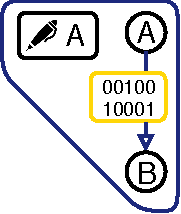
\includegraphics[width=.4\linewidth]{trustchain/assets/tutorial_1}
		\caption{An micro-record, created and signed by user $ A $. It captures an interaction (resource exchange) between users $ A $ and $ B $.}
		\label{fig:trustchain_tutorial_1}
	\end{subfigure}%
	\begin{subfigure}[t]{.33\textwidth}
		\centering
		\captionsetup{width=.89\linewidth}
		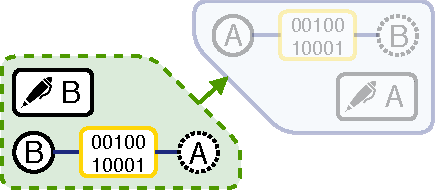
\includegraphics[width=.46\linewidth]{trustchain/assets/tutorial_2}
		\caption{Another micro-record, created and signed by user $ B $, that points to and confirms the micro-record created by user $ A $.}
		\label{fig:trustchain_tutorial_2}
	\end{subfigure}%
	\begin{subfigure}[t]{.33\textwidth}
		\centering
		\captionsetup{width=.93\linewidth}
		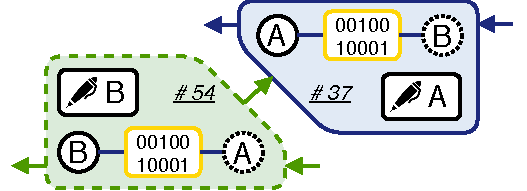
\includegraphics[width=.7\linewidth]{trustchain/assets/tutorial_3}
		\caption{To ensure tamper-proofness, each micro-record references the previous micro-record in the personal ledger of a user.}
		\label{fig:trustchain_tutorial_3}
	\end{subfigure}
	\caption{Storing a bilateral interaction in \ModelName{} using two micro-records.}
	\label{fig:trustchain_tutorial}
\end{figure*}

To show the matureness of \ModelName{}, we leverage our accounting mechanism to record bandwidth exchange in our Tor-like overlay and refuse services to free-riders during periods of congestion.
Our 36-months measurements has resulted in over 120 million micro-records, created by over \TrialUsers{} users.
%This large-scale trial is a key milestone in our ongoing \enquote{bandwidth-as-a-currency} research.
The main contribution of this work is tri-fold:
\begin{enumerate}
	\item \ModelName: a mechanism for micro-accounting in large shared-resource systems (Section~\ref{sec:micro_accounting} and~\ref{sec:system_architecture}).
	\item An evaluation of \ModelName{}, revealing linear scalability and fraud detection times within seconds (Section~\ref{sec:implementation_evaluation}).
	\item A large-scale deployment trial with \ModelName, addressing free-riding in our Tor-like overlay (Section~\ref{sec:deployment}).
\end{enumerate}

%We believe that the tragedy of the Internet commons can be solved through trust-based mechanisms.
%In this work, we build the required digital infrastructure and tools for sustainable community management on the Internet: accounting mechanisms, reputation algorithms, allocation policies.
%All presented components have been evaluated and tested through field trials with real users, using our academic software named Tribler.
%Tribler is the result of 15 years of engineering effort and has been downloaded by over 1.x million users.

% Possible system attacks:
% Free-riding
% Misreporting
% Collusion
% White-washing

\section{Problem Description}
The main challenge is to design and implement a mechanism for micro-accounting of community interactions in large shared-resource systems.
To this end, we formulate three requirements and clarify on the problems we have to address.
%We now elaborate on two requirements for this mechanism and clarify on the problems we have to address.

First, our mechanism must be able to \emph{detect and punish the manipulation} of created records.
Peers in shared-resource systems have a natural incentive to tamper with their prior records to inflate their social standing, or by hiding unfavourable records~\cite{meulpolder2009bartercast}.
Our mechanism must detect record tampering and punish the adversarial peers accordingly, e.g., by refusing them services.
We consider dealing with the recording of interactions that have not actually occurred in the system outside the scope of this work.

Second, our mechanism must \emph{scale} when the network population and number of interactions grow.
Blockchain is increasingly being used to store process transactions without middleman.
However, blockchain in general suffer from scalability limitations since they establishes a network-wide consensus on the entire transaction set~\cite{vukolic2015quest}.
Scalability concerns are partially addressed by layer two solutions that maintain off-chain channels between users, e.g., state channels~\cite{mccorry2019pisa}.
Yet, such approaches still rely on a \enquote{primary} blockchain for dispute resolution and are unsuitable for any-to-any interactions since there is not always an available channel to another peer.
We require that our mechanism is scalable and avoids the need for global consensus.

Third, we require that our mechanism does not rely on \emph{centralized} authorities.
Centralized services pose a single point-of-failure and are prone to manipulation.
Instead, fully decentralized mechanisms are less vulnerable to targeted attacks, tend to scale better and are a good architectural fit with many existing shared-resource systems, e.g., BitTorrent.


%Even though it is impossible to establish that the interaction embedded in a record has actually occurred, our micro-accounting mechanism should be able to handle record manipulation.

% Problem 1: detect manipulation
% Problem 2: avoid reliance on TTP

\section{Micro-Accounting of Interactions}
\label{sec:micro_accounting}
We now describe how the global data structure of \ModelName{} is structured.
In shared-resource systems and \ModelName{}, an interaction indicates the contribution or consumption of resources, e.g., the exchange of a file.
Figure \ref{fig:trustchain_tutorial} outlines how a bilateral interaction is accounted with two distinct \emph{micro-records}.
Figure \ref{fig:trustchain_tutorial_1} highlights one micro-record created by user $ A $, describing an interaction between $ A $ and $ B $.
%A transaction is a generic description of any interaction between users, for instance, making an agreement or recording a trade.
%We consider a transaction to be the result of \emph{any} interaction between users, like transferring assets or recording agreements. %We intentionally consider a transaction to be a description of any interaction between two users.
% As a result, it can describe almost every interaction between two or more users, like asset transfers or generic agreements.
The micro-record contains the digital identity of both the creator and the interaction counterparty.
The creator of the micro-record digitally signs the micro-record and includes the signature.
%It also confirms that both parties agree with the transaction itself.
%Digital signatures can be effectively verified by others.
The micro-record is persisted and sent to the counterparty.
%Each transaction has a \emph{type} field, indicating its purpose.
%Blocks are linked together by a (hash) pointer that points to the prior block in each individual ledger.
%Both transacting parties digitally sign the transaction they are involved in by using any secure digital signing algorithm (TrustChain uses the ECDSA algorithm).
%These digital signatures are included in a block, which ensures that participation by both parties is irrefutable.
%It also confirms that both parties agree with the content within the transaction.
%Others can efficiently verify digital signatures in blocks since the digital identities of both interacting parties (their public keys) are also included in a block.
%After all required signatures have been added to a block, the block is appended to the individual ledgers of the two interacting parties and committed to their local databases.
%TrustChain also allows unilateral transactions without any counterparty.
%The block with a unilateral transaction is only signed by the issuing party and then committed to their individual ledger.

When the counterparty receives the micro-record,t it confirms the incoming micro-record by creating a new one, see Figure~\ref{fig:trustchain_tutorial_2}.
%We extend the micro-record structure in Figure~\ref{fig:trustchain_tutorial_1} and counterparties to \emph{confirm} the record, resulting in bilateral agreements.
Figure~\ref{fig:trustchain_tutorial_2} highlights a micro-record, created and signed by $ B $, that confirms the micro-record created by $ A $.
This new micro-record also contains a hash pointer to the micro-record created by $ A $.
After its creation, $ B $ persists and sends the confirming micro-record to $ A $.
Both parties are now in possession of two linked micro-records that together prove agreement of both parties on an interaction.

%Note how the blockchain structure in Figure \ref{fig:trustchain_tutorial_2} allows user $ A $ to modify blocks in their individual ledger without being detected by others.
%In particular, $ A $ can reorder the blocks in its individual ledger since validity can quickly be restored by recomputing all hashes.
%In most blockchain applications, the global consensus mechanism prevents this kind of manipulation.
To ensure tamper-proofness, we link micro-records created by the same user together such that they form a hash chain.
Specifically, we extend each micro-record with an additional hash pointer that points to the prior micro-record in the personal ledger of an individual, incrementally ordered by creation time.
This is visualized in Figure \ref{fig:trustchain_tutorial_3}.
Each micro-record now has a sequence number that indicates its position in the personal ledger.
As a result, each user maintains their own local chain which contains all transactions in which they have participated.
This sets \ModelName{} apart from the structure of traditional blockchains, where the entire network reaches consensus on a single, linear ledger.
%Each block now has exactly two incoming and two outgoing (hash) pointers, except for the last block in an individual ledger, which only has two incoming pointers.

\begin{figure}[t]
	\centering
	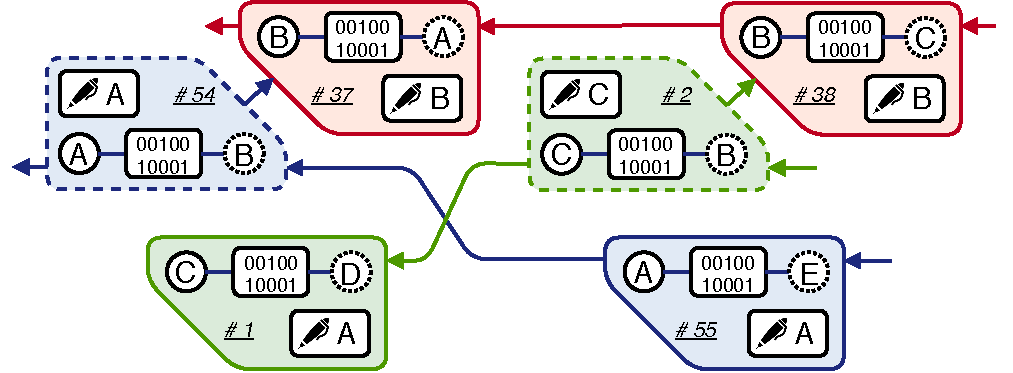
\includegraphics[width=\linewidth]{trustchain/assets/fullchain}
	\caption{A part of the \ModelName{} DAG with three users and seven micro-records. One micro-record is unconfirmed.}
	\label{fig:fullchain}
\end{figure}

Repeated interactions and therefore creation of micro-records yields the directed acyclic graph (DAG) structure as shown in Figure \ref{fig:fullchain}.
Figure \ref{fig:fullchain} shows seven micro-record, created by three users.
Micro-records in the same personal ledgers have the same colour.
When two parties transact and create a block, their personal ledgers essentially become entangled.
This accounting approach is lightweight: recording a bilateral interaction only requires two signatures and the exchange of two micro-records.
%This property makes fraud impractical to hide since a counterparty is able to proof malicious activities by revealing his block with the disputed transaction.

We now elaborate how \ModelName{} deals with fraud, specifically the manipulation of records.
\ModelName{} orients around fraud \emph{detection} instead of \emph{prevention}.
We argue this is a reasonable assumption since shared-resource systems can usually tolerate low amounts of fraud for short time periods.
In \ModelName{}, users continuously request micro-records from others.
This exchange process enables efficient detection of different types of fraud.
Modifications of the personal ledger, like reordering or removing micro-records, can now be detected and proven by other users since this will invalidate the hash pointers.
To prove this fraud to others, a user can broadcast the original and manipulated micro-records.
A particular challenging kind of fraud is \emph{forking}, where a malicious user creates two micro-records with the same sequence number but differing content and counterparties.
Only when a user discovers both conflicting micro-records, this fraud can be revealed to the network.
In Section~\ref{sec:fraud_detection_experiment} we experimentally show that forking can be detected within seconds.
%To prove this fraud, the transaction counterparty reveals both the correct block and the invalid block created by $ A $.

\section{System Architecture}
\label{sec:system_architecture}
%We present the components of our middleware, which is visualized in Figure~\ref{fig:system_architecture}.
%We consider peer-to-peer communities without centralized server.
%We also deem threats at the network layer, such as the Sybil Attack and the Eclipse Attack, outside scope of this work.

%\subsection{Underlying Model for Resource Management}
%Figure~\ref{fig:model} shows the underlying model of our middleware.
%This model is inspired by prior work on deterring free-riders in BitTorrent networks based on reputation, and consists of three components~\cite{seuken2010accounting,meulpolder2009bartercast}.
%An \emph{accounting mechanism} (see Section X) stores all resource contributions and consumptions by agents.
%These actions are embedded in tamper-proof and light-weight records, and shared with other individuals in the network.
%Each individual collects records from others, eventually building a local database.
%These records are then passed to a \emph{reputation algorithm} that determines the trustworthiness of individuals it knows about.
%Even though accounting mechanisms and reputation mechanisms share similarities, they are incomparable as discussed in the work of Seuken et al.~\cite{seuken2010accounting}.
%There exists a large number of decentralized reputation algorithm.
%The output of the reputation algorithm is a mapping from the identity of individuals to a trust score.
%These trust scores are used by the \emph{allocation policy} to provide access to some common good.
%The interactions following the allocation are accounted and public, and influence subsequent trust scores.
%For example, if a peer $ A $ downloads from another peer $ B $, the trust score of peer $ B $ most likely increases whereas the scores of peer $ A $ decreases.

We devise a system architecture around our micro-accounting model, see Figure~\ref{fig:system_architecture}.
We now elaborate its components.
%We also demonstrate how resource-sharing applications can leverage the described system architecture and leverage \ModelName{} for resource accounting.

\textbf{Communication Layer.}
The communication layer passes incoming (serialized) micro-records to the record manager and routes outgoing serialized micro-records to their intended destination.
This layer can be realised using existing frameworks to build peer-to-peer overlay networks, e.g., libp2p.
We assume that defences against network threats, e.g., the Sybil and Eclipse attacks, are addressed by the communication layer.

\textbf{Record Manager.}
The record manager is the central coordinator of our micro-accounting mechanisms.
It serializes and deserializes outgoing, respectively incoming micro-records and coordinates the validation process of micro-records.
When micro-records arrive from the network, the record manager first checks if it has been received before.
If not, it schedules the micro-record for validation.

\begin{figure}[b]
	\centering
	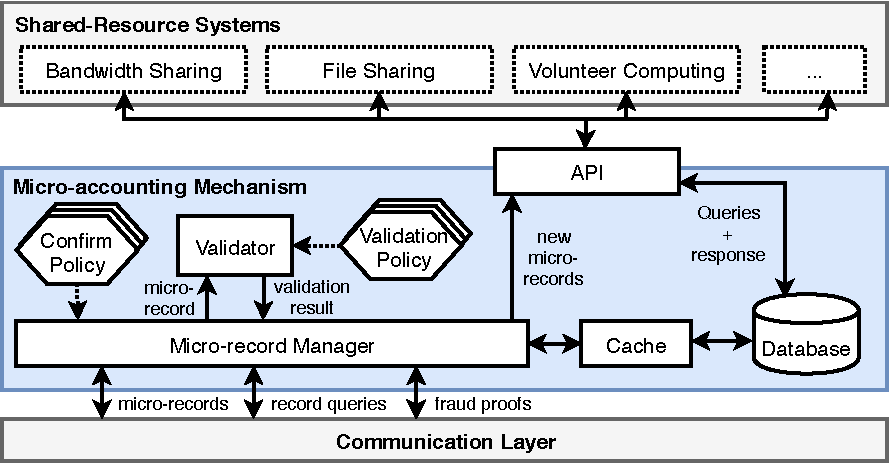
\includegraphics[width=\linewidth]{trustchain/assets/system_architecture}
	\caption{The system architecture of \ModelName{}.}
	\label{fig:system_architecture}
\end{figure}

\textbf{Validator.}
The validator assesses the validity of incoming micro-records.
We distinguish between validation on \emph{record-level} and \emph{data-level}.
Validation on record-level verifies the whether the micro-record itself is valid, e.g., whether it contains a valid digital signature and whether the micro-record is in alignment with other known micro-records in the personal ledger.
These validation rules are application-agnostic.
Validation on data-level verifies integrity of the micro-record with respect to an application context.
Note that the validator might not have sufficient information to validate an incoming micro-record and therefore can request more micro-records in the same personal ledger.
Developers can implement different \emph{validation policies} for different micro-record types.
When the validator determines a fraud attempt, the record manager disseminates the fraud proof, consisting of multiple micro-records, in the network.

When a user $ A $  receives a (valid) incoming micro-record specifying an interaction with $ A $, the record manager invokes a \emph{confirm policy} that predicates whether $ A $ should create a confirming micro-record.
Whether $ A $ should confirm an incoming micro-record could consider application-specific information e.g., whether an interaction has really happened.

%\begin{algorithm}[b]
%	\SetAlgoLined
%	\small
%	\KwData{Micro-record \emph{R}, database \emph{db}}
%	\lIf{$ R $.$sequence\_number < 1 $}{\Return{} \textbf{false}}
%	\lIf{f}{\Return{} \textbf{false}}

%	\caption{The validation of a micro-record}
%\end{algorithm}

\textbf{Persistence.}
Valid micro-records and fraud proofs are persisted in a database.
When validity of a micro-record has been determined, the record manager passes the record to the \emph{record cache}.
The record cache stores intermediate records for quick lookup when receiving a query for micro-records in ones personal chain.
When starting \ModelName{}, it pre-loads the micro-records of the operating user in the cache.
The record cache interacts with the micro-record database for the retrieval and storage of micro-records.

\textbf{Fraud Management.}
When the validator detects a fraud attempt, or when receiving an incoming fraud proof from the network, the fraudster is punished according to a \emph{fraud policy}.
For example, a fraud policy in a bandwidth sharing application could decide to not serve the fraudster for some time.
Also depending on the fraud severity, different applications might demand different fraud policies.

\section{Implementation and Evaluation}
\label{sec:implementation_evaluation}
We implement the presented micro-record model (Section~\ref{sec:micro_accounting}) and system architecture (Section~\ref{sec:system_architecture}) in the Python 3 programming language in around 3.000 lines of code.
We leverage our existing networking library as communication layer, supporting the engineering of decentralized overlays, NAT traversal and authenticated messaging.\footnote{Omitted for double-blind review.}
We adopt an event-driven programming model using the \texttt{asyncio} library.
For efficiency, we use the UDP protocol to exchange micro-records and keep track of outstanding record queries using request stores and timeouts.
The full implementation of \ModelName{}, including documentation and unit tests, are on GitHub.

We evaluate \ModelName{} on our nation-wide university cluster which hardware specifications can be found online.
Our evaluation answers the following two questions: (1) what is the maximum rate at which micro-records can be created when the network size grows? and (2) how fast can forking be detected with varying network sizes?

\begin{figure}[t]
	\centering
	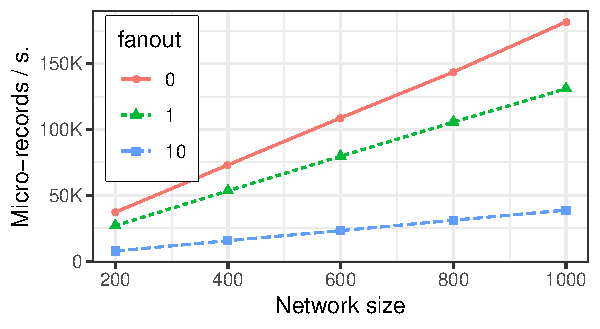
\includegraphics[width=\linewidth]{trustchain/assets/scalability}
	\caption{The maximum speed at which confirmed micro-records can be created in \ModelName{} while varying the network size and broadcast fanouts.}
	\label{fig:scalability}
\end{figure}

\subsection{Scalability}
We explore the scalability of \ModelName{} by having each peer create a new micro-record at a fixed interval.
This micro-record is targeted at another random peer.
We systematically explore the maximum throughput for different network sizes and broadcast fanout (the number to which a new micro-record is sent after creation).
Each peer creates a micro-record targeted at another random peer, and the other peer always confirms incoming micro-records.
After creating a micro-record, it is disseminated to $ f $ random users (we call $ f $ the fanout).
We persist all micro-records in memory.
For differing network sizes ($ n $) and fanout ($ f $), we determine the maximum rate at which confirmed micro-records can be created during a 30-seconds experiment run.

The results of our experiment are presented in Figure~\ref{fig:scalability}, with the network size on the horizontal axis and the maximum micro-record creation rate on the vertical axis.
\ModelName{} is able to create 181'729 confirmed micro-records per second with 1'000 peers and $ f = 0 $.
During this run, the average bandwidth usage per peer is 121 KB/s.
A higher fanout negatively affects the throughput: with $ f = 10 $ and $ n = 1'000 $, \ModelName{} outputs 38'810 confirmed micro-records per second.
Figure~\ref{fig:scalability} also hints at linear scalability when the network size grows.
Our current implementation is single-threaded and the achievable throughput can still be improved by leveraging parallelism.
The current throughput of \ModelName{}, however, is sufficient for deployed shared-resource applications.

\begin{figure}[t]
	\centering
	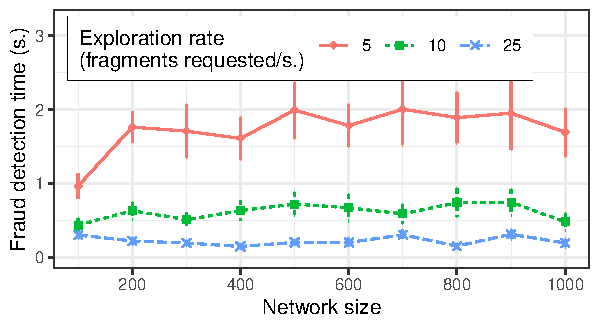
\includegraphics[width=\linewidth]{trustchain/assets/fraud_detection}
	\caption{The time until a fork in a personal ledger is detected in \ModelName{}, while varying the network size and micro-record request rates.}
	\label{fig:fraud_experiment}
\end{figure}

\subsection{Fraud Detection}
\label{sec:fraud_detection_experiment}
We evaluate the efficiency of detecting forking fraud in \ModelName{} by measuring the time between committing the fraud and its initial detection.
Our focus is on the \emph{forking of a personal ledger}, which requires discovery of micro-records in two distinct personal ledgers in order to be revealed.

The global rate at which transactions are made is fixed to 100 transactions per second.
Users create micro-records targetting other random users.
During the experiment, each peer explores others' personal ledgers by continuously querying their latest micro-record, and attempts to detect fraud.
At the start of each experiment, we selected one peer to perform exactly one double spend attack.
This peer re-uses the sequence number of the latest micro-record (forking) with 20\% probability.
We measure the interval between initiation of the fraud and its first detection (upon which the proof can be spread in the network).
We vary the rate at which users request micro-records from each other.
We consider request frequencies of 5, 10 and 25 (where 5 means that each user will request a micro-record from five other users every second).
For each combination of network size and ledger exploration rate, we run the experiment 20 times.

The results are given in Figure \ref{fig:fraud_experiment}.
The horizontal axis denotes the network size and the vertical axis shows the time interval between performing the forking and its detection.
The errors bars show one standard deviation of uncertainty.
Figure \ref{fig:fraud_experiment} shows that faster querying of micro-records increases the speed of fraud detection, at the expense of increased resources usage (bandwidth and CPU utilization).
We observe that the variation of fraud detection speed is higher when exploring personal ledgers at a lower rate.
Interesting is that effectiveness of fraud detection shows comparable results when the network size increases.
Our reasoning for this is as follows: although the specific double spend is more "hidden" in the network, there is also more ongoing effort to detect it.
This experiment shows that forking of a personal ledger can be detected within mere seconds and 1'000 active peers.

\section{Preventing Free-riding at Scale}
\label{sec:deployment}
We now present our large-scale deployment trial to prevent free-riding behaviour in our academic peer-to-peer client named \Tribler{}, which is downloaded by over 1.5 million users.
We integrate \ModelName{} in our Tor-like overlay that onion-routes BitTorrent traffic through relay and exit nodes and thus hides the identity of the downloader.
This overlay suffers from a lack of exit nodes, leading to frequent congestion and degradation of anonymous download speed for all active users.
The aim of our trial is to prevent a tragedy-of-the-commons and address free-riding behaviour by having users that contributed to the network as relay or exit node receive preferential treatment during periods of congestion.

\begin{figure}[t]
	\centering
	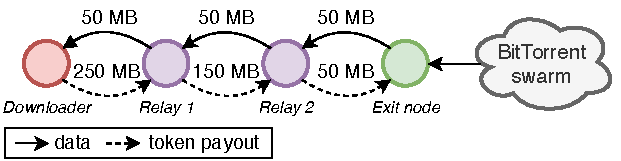
\includegraphics[width=\linewidth]{trustchain/assets/payouts}
	\caption{Accounting an anonymous 50MB BitTorrent download using \ModelName{} and a single two-hop circuit.}
	\label{fig:payouts}
\end{figure}

\subsection{Accounting Bandwidth Transfers}
Each peer can accumulate \emph{bandwidth tokens} by operating a relay or exit node and spend earned tokens by downloading content.
Figure~\ref{fig:payouts} show how \ModelName{} accounts bandwidth transfers in \Tribler{}, when downloading a 50 Megabyte file over a circuit with two relay nodes.
After the download has completed, the downloader creates a micro-record that transfers 250MB to the first relay node (MB is our unit for).
The first relay node then transfers 150MB to the next relay node, earning 100MB.
The rationale behind our payout scheme is that we reward relay nodes for encrypting and decrypting incoming and outgoing traffic respectively.
Exit nodes are rewarded for encrypting outgoing traffic.
Each micro-record in a personal ledger contains the amount of transferred token, and the current token balance.
We payout anonymous transfers of at least 1MB.

Our mechanism records data transfers through a circuit.
We plan on addressing privacy concerns by having a node aggregate and delay payouts, discussed in the work of Palmieri et al. ~\cite{palmieri2015paying}.
Still, our accounting mechanism does not leak the identity of a downloader to others, nor the data being exchanged.
To address the uncontrolled minting of bandwidth tokens, we are currently implementing a Sybil-resistant reputation mechanism~\cite{otte2017trustchain}.
Finally, relays that do not forward the payout to the next hop, will be blacklisted by the previous hop, affecting their opportunity to earn bandwidth tokens.

To fairly allocate relay and exit node traffic, we implement a slot-based mechanism where each circuit consumes an available slot.
We distinguish between \emph{random} slots and \emph{competitive} slots.
When a circuit initiation request arrives, \Tribler{} first determines if there is a random slot available and if so, assigns the new circuit to it.
If not, \Tribler{} queries the bandwidth token balance of the circuit initiator $ i $ by requests the latest micro-record in its personal ledger.
\Tribler{} now checks eligibility for a competitive slot.
If there is a free competitive slot, it assigns the new circuit to it.
When all competitive slots are filled, the circuit of the initiator with the lowest amount of bandwidth tokens, say $ p $, is destroyed if the token balance of $ i $ is higher than the token balance of $ p $.
As an effect, peers with a higher token balance have more chance to claim a competitive slot in periods of congestion, compared to free-riders, and thus they experience higher anonymous download speeds.

\begin{figure}[b]
	\centering
	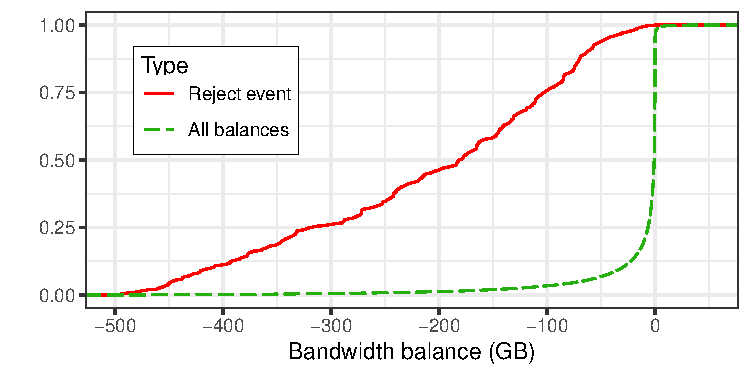
\includegraphics[width=\linewidth]{trustchain/assets/exit_node_rejects}
	\caption{ECDF showing the distribution of bandwidth token balances users and individual rejects events at exit nodes.}
	\label{fig:exit_node_rejects}
\end{figure}

\subsection{Refusing Services to Free-Riders}
We implement the aforementioned mechanisms in \Tribler{} and release a new version of our software.
We setup a crawler that fetches \ModelName{} micro-records from random users in the network.
The crawler selects a random user in the network every two seconds, and requests missing micro-records in their personal ledger.
This has resulted in more than 120 million micro-records, created by over \TrialUsers{} individuals during 36 months.
In addition, our crawler discovered 127'135 instances where a personal ledger was forked.
Overall, this deployment trial proves the matureness of \ModelName{}.

To evaluate the effectiveness of our bandwidth scheduling mechanism, we deploy 48 additional exit nodes and monitor them for two weeks.
Each process has 10 random slots and 20 competitive slots available, resulting in a total of 1'440 slots.
We log the balance when a circuit initiator is unable to get a slot at one of our exit nodes.
In total, we logged over 1.2 million reject events.

Figure~\ref{fig:exit_node_rejects} shows the ECDF with the bandwidth token balances of all users (dotted green line) and the balances of reject events (solid red line).
We filter out all users and reject events with balances higher than 50GB or lower than -500GB.
The median token balance of all users is -713MB and the median token balance of reject events is -181.4GB, demonstrating that our mechanism effectively targets users with low balances.
We conclude from our deployment trial that \ModelName{} is an effective at detecting and addressing free-riding behaviour in \Tribler{}.

%\begin{figure}[t]
%	\centering
%	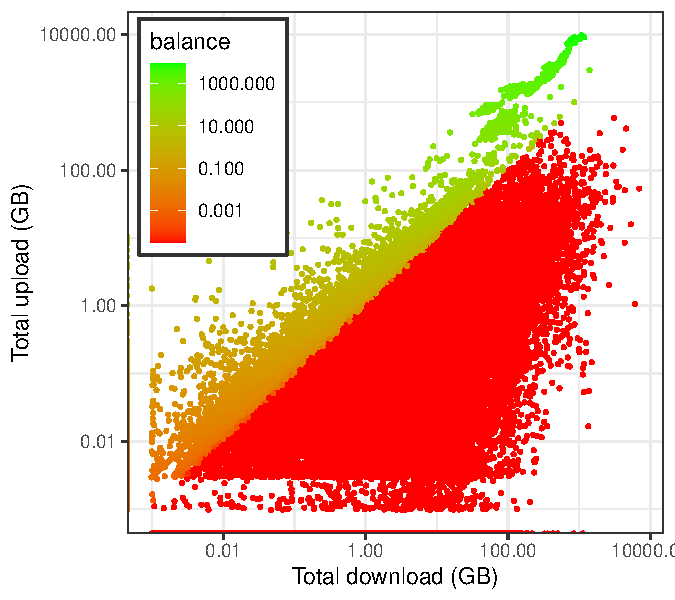
\includegraphics[width=\linewidth]{assets/balances_scatter}
%	\caption{The bandwidth balances of users in Tribler. Users with a balances less than 5GB are marked red.}
%	\label{fig:balances}
%\end{figure}

\section{Related Work}
Motivated by the potential of blockchain technology, there have been proposals for a lightweight distributed ledger.
Vegvisir is a partition-tolerant blockchain designed for Internet-of-Things~\cite{karlsson2018vegvisir}.
PeerReview is an accountability system to record message exchange between peers, dedicated witnesses to detect whether a peer deviates from the protocol~\cite{haeberlen2007peerreview}.
Otte et al., present TrustChain, a Sybil-resistant reputation mechanism that uses a decentralized accounting mechanism~\cite{otte2017trustchain}.
However, peers in TrustChain cannot engage in the creation of multiple records simultaneously, limiting throughput and enabling a denial-of-service attacks.
Crosby et al., present a tamper-evident log, built for the logging of system events~\cite{crosby2009efficient}.

% Tor accounting
There has been considerable effort to incentivize Tor relay and exit node operators.
One of the earlier approaches is Gold Star where directory servers keep track of users providing good services to the community~\cite{dingledine2010building}.
Other approaches like BRAIDS and LIRA, reward relay and exit nodes with credits that can be redeemed for prioritized traffic~\cite{jansen2010recruiting,jansen2013lira}.
These solutions are relying on a centralized bank or a group of semi-trusted nodes for credit management.
More recent solutions leverage micro-payments with cryptocurrencies.
TorCoin proposes a mechanism where relay and exit nodes \enquote{mine} a Bitcoin-derived cryptocurrency~\cite{ghosh2014torpath}.
TorCoin, however, relies on a centralized server for circuit management.

Several shared-resource applications based on blockchain use monetary incentives to provide community services, e.g., storage (Filecoin~\cite{benet2018filecoin}), Tor traffic (TorCoin~\cite{ghosh2014torpath}) and BitTorrent bandwidth (BitTorrent token).
These systems store all community interactions on a single, linear ledger that is secured with global consensus.

\section{Conclusion}
We have presented \ModelName{}, a micro-accounting mechanism to free-riding in shared-resource systems.
Our model uses micro-records and hash pointers to capture bilateral agreements such as the exchange of a file.
Since each user maintains a tamper-evident personal ledger, manipulation can be detected by others by the continuous exchange of micro-records.
We have implemented \ModelName{} and demonstrated with experiments that our mechanism is highly scalable and detects even the most challenging kind of fraud (forking) within seconds.
A large-scale deployment trial, involving over \TrialUsers{} users, demonstrated how \ModelName{} is used to address bandwidth free-riding in our peer-to-peer software.